\epigraph{But can it run Crysis?}{Anon}

\minitoc

% Why GPUs ?

\section{Why is efficient threading tricky on CPUs ?}

So far we have almost exclusively focused on programming central processing units (CPU) in serial with C, then with OpenMP annotated C for multithreading to exploit multiple CPU cores, and subsequently distributed computing to run on multiple CPUs by calling MPI from C. In some cases we have only seen modest performance gains from multithreading. Furthermore, we have discussed the difficulty of persuading the compiler to generate vector instructions that instruct the CPU SIMD units to perform multiple arithmetic operations simultaneously per core.  The compiler is cautious to introduce these instructions because of the requirement that it can guarantee all data inputs and outputs to the vector instructions need to be aligned to appropriate memory page boundaries and that the full vector width can be exploited in the calculation. 

I have personally observed the progression in vector instruction sets for Intel CPUs. Recalling the \href{https://en.wikipedia.org/wiki/MMX_(instruction_set)}{MMX} vector extensions released in 1997, the Streaming SIMD Extensions (\href{https://en.wikipedia.org/wiki/Streaming_SIMD_Extensions}{SSE}) released in 1999, the enlarged instructions setextensions \href{https://en.wikipedia.org/wiki/SSE2}{SSE2}, \href{https://en.wikipedia.org/wiki/SSE3}{SSE3}, \href{https://en.wikipedia.org/wiki/SSE4}{SSE4}, followed by the Advanced Vector Extension \href{https://en.wikipedia.org/wiki/Advanced_Vector_Extensions}{AVX}, the sequel \href{https://en.wikipedia.org/wiki/Advanced_Vector_Extensions}{AVX2}, and the even wider SIMD follow on \href{https://en.wikipedia.org/wiki/Advanced_Vector_Extensions}{AVX-512}. Each of these vector instruction extensions includes specialized functions for SIMD instructions of hardware specific vector operations. From a practical point of view it is not an attractive prospect to write code that targets the contemporary vector instruction knowing full well that it will need to be updated for the next CPU SIMD instruction set\footnote{There is some useful information \href{https://www.agner.org/optimize/}{here} about how to target specific families of CPU processors.}. It is possible to write code where the vector operations are isolated to small parts of the code, but the requirements of vector operations enforce global requirements on data alignment.

Many of the problems with CPU vector SIMD units boil down to their being retrofitted into the well established x86 core architecture. An optimizing compiler has to decide whether it is possible to engage the SIMD processor for a set of operations, for instance bulk processing arithmetic iterations from chunks of loop iterations. The compiler has to verify that all data is properly aligned, that there is no loop carried dependency, and apply heuristic models to estimate whether the vectorized operation would be faster than just using sequential operations. Most recently it has come to light that some late generation Intel CPUs throttle clock frequency when using the wide AVX-512 operations \href{https://blog.cloudflare.com/on-the-dangers-of-intels-frequency-scaling/}{reducing the performance below expectations}. In summary: the vector extension sets for Intel CPUs are a moving target; it is difficult to persuade CPU compilers to automatically generate code for the SIMD units; even if the compiler can be persuaded to vectorize code the CPU may reduce the CPU clock frequency.

\section{Graphics processing units as an alternative to CPUs}

The CPU is fortunately not the only game\footnote{See what we did there?} in town for performing calculations on a computer. The popularity of home computers, video games, game consoles, and PC gaming in the 80s and 90s drove the parallel\footnote{Unavoidable, really.} development of graphics processing units (GPUs). Typical early GPUs were highly specialized processors that were designed to efficiently render polygonal 3D scenes into a display buffer at acceptably playable resolution and framerate. Manufacturers including ATI (now AMD), NVIDIA, SGI, Sony and others produced GPUs starting in the early 1990s. Their GPUs were used to accelerate the rendering of graphics in a wide range of settings including professional workstations (SGI), PC desktops (ATI, NVIDIA, 3dfx), and game consoles (Sega, NVIDIA, AMD). More recently laptops and cell phones have crucially depended on GPUs to deliver high resolution (4K) displays for relatively low energy overhead given that these are battery powered devices.

The use cases envisioned for GPUs initially was very different to CPUs. In the 1990s the former only had to excel at rendering graphics in a timely fashion whereas the latter was expected to be capable of general purpose computing tasks encompassing business applications including payroll, word processing, spreadsheets, CAD, CAE, databases, and countless other user facing applications.  The GPU had to mediate between the CPU and the display, but the CPU had to also coordinate physical storage (CD drive, hard drive, tape drive), network, user interface (mouse, keyboard, trackball\ldots), and a myriad of attached devices.  

The specialized tasks of early GPUs enabled the chip designers to build computational cores with lower complexity than general purpose CPU cores. Furthermore since the tasks required to color pixels on a display are the same for each pixel it was possible to employ ab initio hierarchical parallelism with the capability to concurrently execute a large number of hardware threads. Each product in the modern NVIDIA GPU lineup consists of multiple compute cores\footnote{NVIDIA calls each GPU core a Streaming Multiprocessor (SM).}. Each compute core is equipped with one or more vector SIMD arithmetic logic units, i.e. floating point units.

\begin{figure}[htbp!]
    \centering
    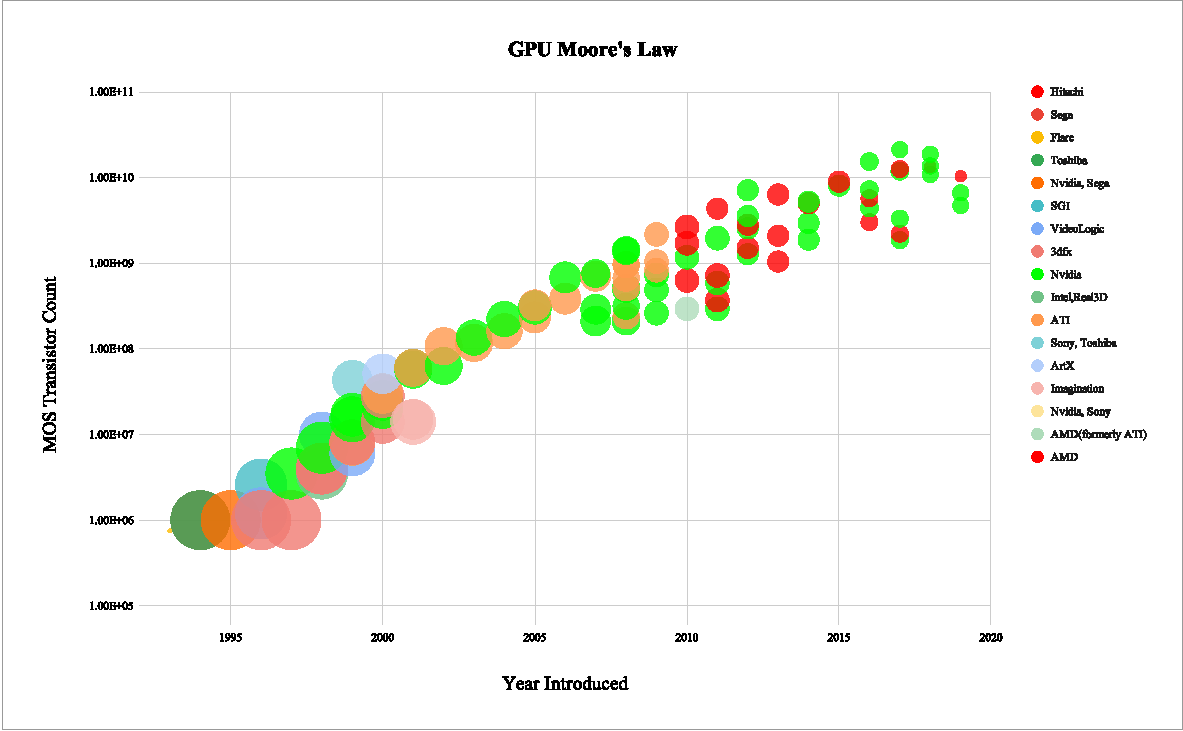
\includegraphics[width=0.85\textwidth]{figures/L24/GPUMooresLaw-crop.pdf}
    \caption{Moore's law for GPUs: data obtained from \href{https://en.wikipedia.org/wiki/Transistor_count}{wiki page on transistor counts}. Nearly thirty years of data show continued exponential increase in transistor counts, with some noticeable dips in the trend. For instance 2013-2015 there were delays in transitioning between 28nm and 14/16nm manufacturing processes. Scatter symbols are scaled by manufacturing process size with the latest AMD GPUs manufactured at 7nm.}
    \label{GPUMooresLaw.fig}
\end{figure}

The progression of GPUs since their inception in the 1990s has been remarkable. For instance he number of transistors used in GPUs has followed a Moore's Law like trend with exponential growth maintained for 20 years as shown in Figure \ref{GPUMooresLaw.fig}, only showing signs of slow down in the 2013-2015 where both NVIDIA and AMD got ``stuck'' at the 28nm manufacturing process due to the technical challenges in transitioning to 14nm. From my personal experience although it might appear that the GPUs did not progress in manufacturing process scale, the manufacturers actually used node improvements in the core microarchitecture and the GPUs did improve in performance during this time. 

\begin{tcolorbox}[width=\textwidth,colback={lightgray},title={Acknowledgement of source for CPU/GPU performance trend data and figures},colbacktitle=yellow,coltitle=blue] 
In the following we include figures sourced from \href{https://www.karlrupp.net/2013/06/cpu-gpu-and-mic-hardware-characteristics-over-time/}{Karl Rupp's webpage} and \href{https://github.com/karlrupp/cpu-gpu-mic-comparison}{his GitHub repository}. His resources include an excellent write up on the trends in GPUs that I strongly recommend you review his commentary. All figures here were regenerated as of 10/06/2019 and are subject to the license agreement \href{https://github.com/karlrupp/cpu-gpu-mic-comparison/blob/master/LICENSE.txt}{here}.
\end{tcolorbox}

Shrinking transistors over time has allowed many more floating point units to be packaged into each GPU. This has seen an increase in peak double precision from  $\mathcal{O}(100)$ GFLOPS/s in the mid 2000s to $\mathcal{O}(10,000)$ GFLOPS/s in 2018 as shown in Figure \ref{GPUFP64trends.fig}. In that Figure it is also clear that the peak performance has plateaued between shrinks of the manufacturing process for transistors, but my experience is that gap between achievable and peak performance narrowing during the plateaus. We also note that chart shows a considerable gap between contemporary CPUs and GPUs.
\begin{figure}[htbp!]
    \centering
    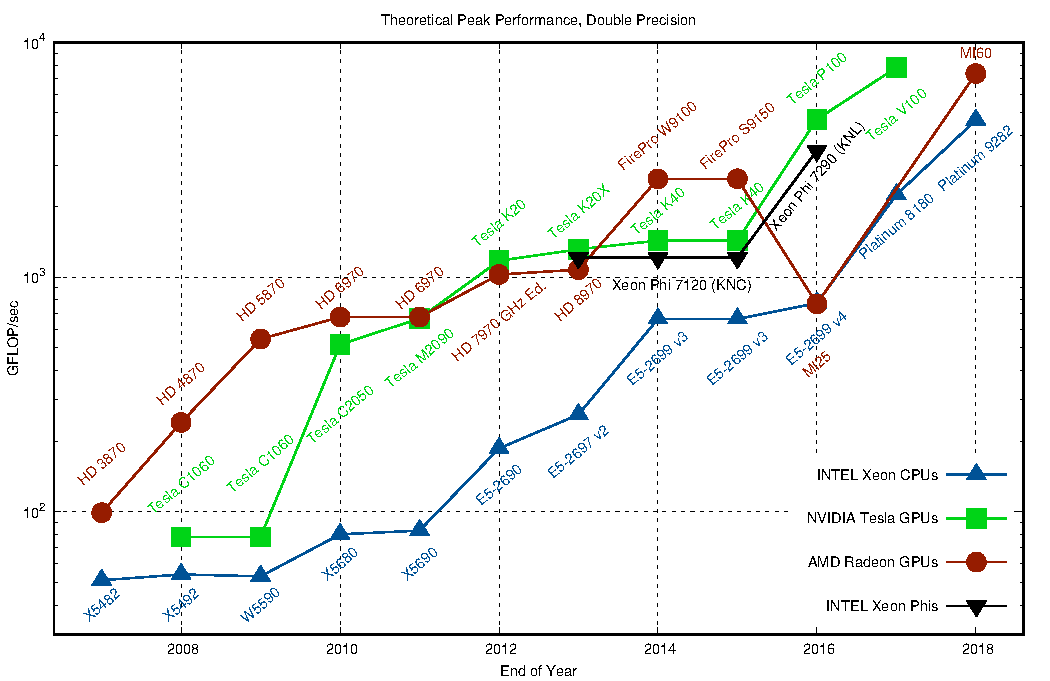
\includegraphics[width=0.75\textwidth]{figures/L24/gflops-dp.pdf}
    \caption{Trend in theoretical peak GPU double precision floating point performance over time. Image generated using Karl Rupp's scripts and data sourced from \href{https://github.com/karlrupp/cpu-gpu-mic-comparison}{his GitHub repository} subject to \href{https://github.com/karlrupp/cpu-gpu-mic-comparison/blob/master/LICENSE.txt}{this license}. }
    \label{GPUFP64trends.fig}
\end{figure}

One thing to keep in mind about the increase in peak performance in GPU double precision performance is that it could be undone if the energy requirement per FLOP increases. Fortunately in Figure \ref{GPUFP64FlopsPerWattTrends.fig} we show that the number of GFLOPS/per Watt by and large has increased over time. Also, there is a considerable energy bonus from using GPUs comparing to CPUs given the gap between their respective GFLOPS/per Watt plot lines.

\begin{figure}[htbp!]
    \centering
    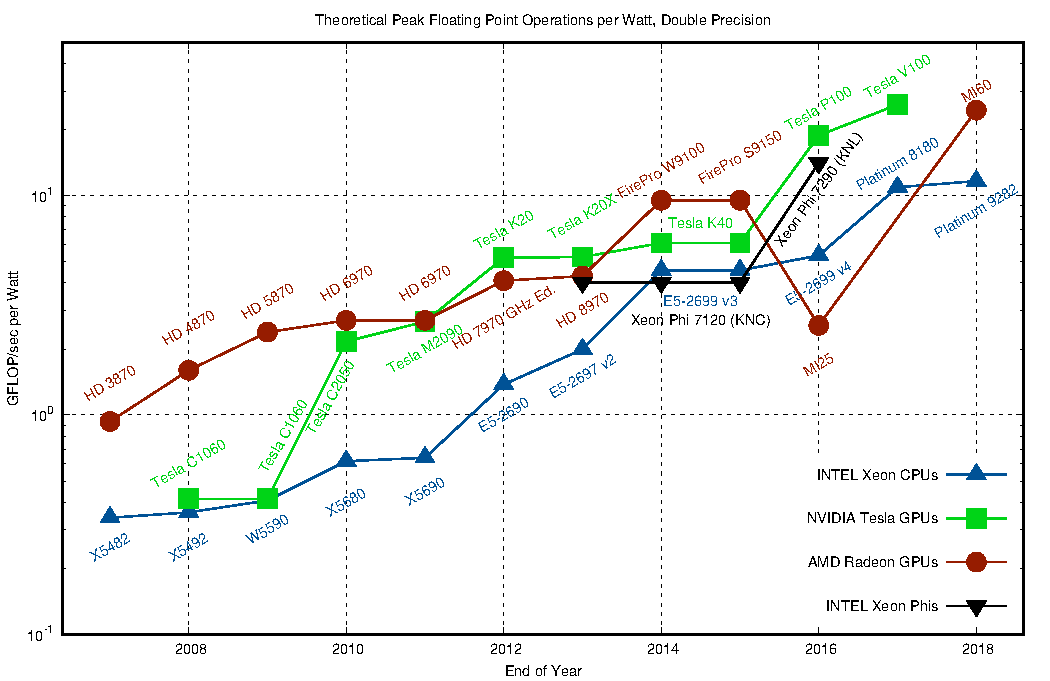
\includegraphics[width=0.75\textwidth]{figures/L24/gflops-per-watt-dp.pdf}
    \caption{Trend in theoretical peak GPU double precision floating point performance normalized by energy consumption over time. Image generated using Karl Rupp's scripts and data sourced from \href{https://github.com/karlrupp/cpu-gpu-mic-comparison}{his GitHub repository} subject to \href{https://github.com/karlrupp/cpu-gpu-mic-comparison/blob/master/LICENSE.txt}{this license}. }
    \label{GPUFP64FlopsPerWattTrends.fig}
\end{figure}

At this point one might ask: assuming that the GPU architectures are eminently scalable\footnote{Assuming that GPU architectures are indefinitely scalable sidesteps several issues that get in the way. For instance although GPUs are typically run at lower clock frequencies than the CPU cousins, the GPUs still require substantial effort to cool and this relies in turn on continuous improvement on processor cooling technology. A second major issue that we will outline in more detail later is that recent GPUs use an L2 cache shared amongst all 80 cores \cite{jia2018dissecting}. History suggests that this arrangement will not scale to a large number of cores given the challenges of coordinating requests from a large number of cores to a shared memory cache system.} what limits the number of cores, the number of floating point units, and thus the overall peak floating point performance ? In Figure \ref{GPUTdpTrends.fig} we show the maximum power consumption (also referred to as \href{https://en.wikipedia.org/wiki/Thermal_design_power}{``Thermal Design Power'' typically shortened to TDP}) for several generations of CPUs and GPUs. For several generations the TDP for GPUs was limited to 250 Watts primarily because the GPUs were connected to the host computer via the PCI-E card interface. The PCI-E standard limits the power consumed by attached devices to 250 Watts, hence the plateau evident in Figure \ref{GPUTdpTrends.fig}. You may also notice the uptick in GPU TDP in 2017 when some NVIDIA Volta V100 GPUs were released with a proprietary hardware interface to the host computer that did not share the same TDP limit as PCI-E.  At the same time you will notice that Intel started to release server CPUs with large increases in their TDP, in part to produce CPUs that are closer in peak floating point performance to the top rated GPUs from AMD and NVIDIA.

\begin{figure}[htbp!]
    \centering
    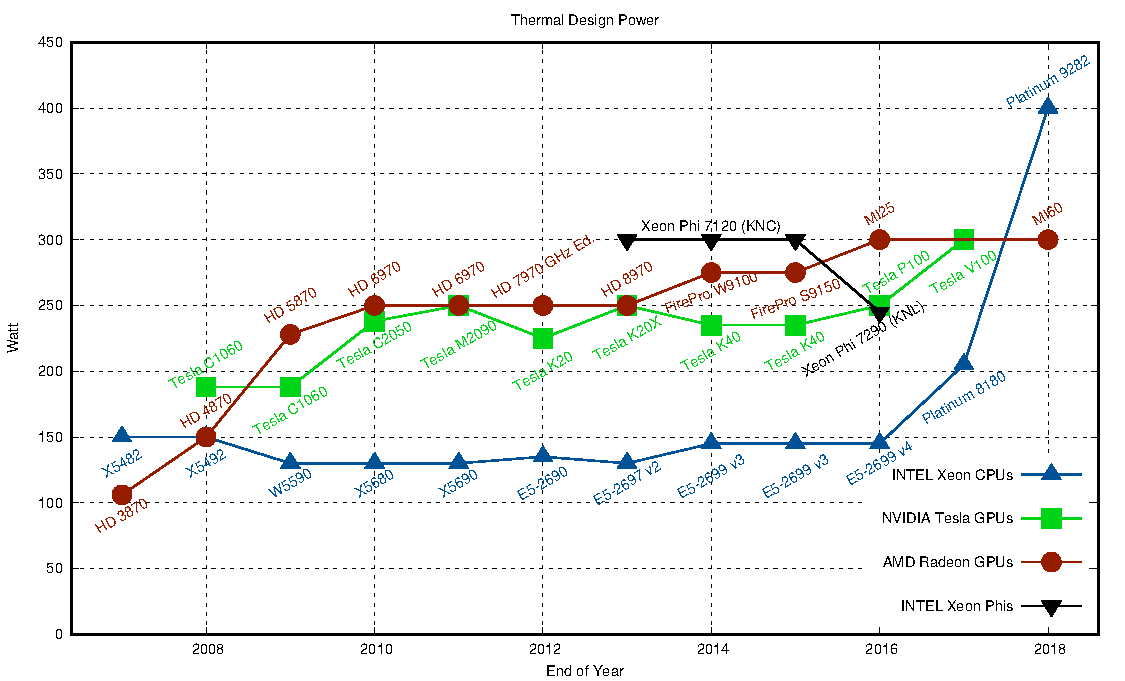
\includegraphics[width=0.75\textwidth]{figures/L24/tdp.pdf}
    \caption{Trend GPU thermal design power maximums over time. Image generated using Karl Rupp's scripts and data sourced from \href{https://github.com/karlrupp/cpu-gpu-mic-comparison}{his GitHub repository} subject to \href{https://github.com/karlrupp/cpu-gpu-mic-comparison/blob/master/LICENSE.txt}{this license}. }
    \label{GPUTdpTrends.fig}
\end{figure}



\section{Contemporary GPU: the NVIDIA Volta V100 GPU}

To make this discussion of GPU architectures concrete we consider the NVIDIA Volta V100 GPU. It has 80 compute cores as illustrated in Figure \ref{NVIDIAV100BlockDiagram.fig}.

\begin{figure}[htbp!]
    \centering
    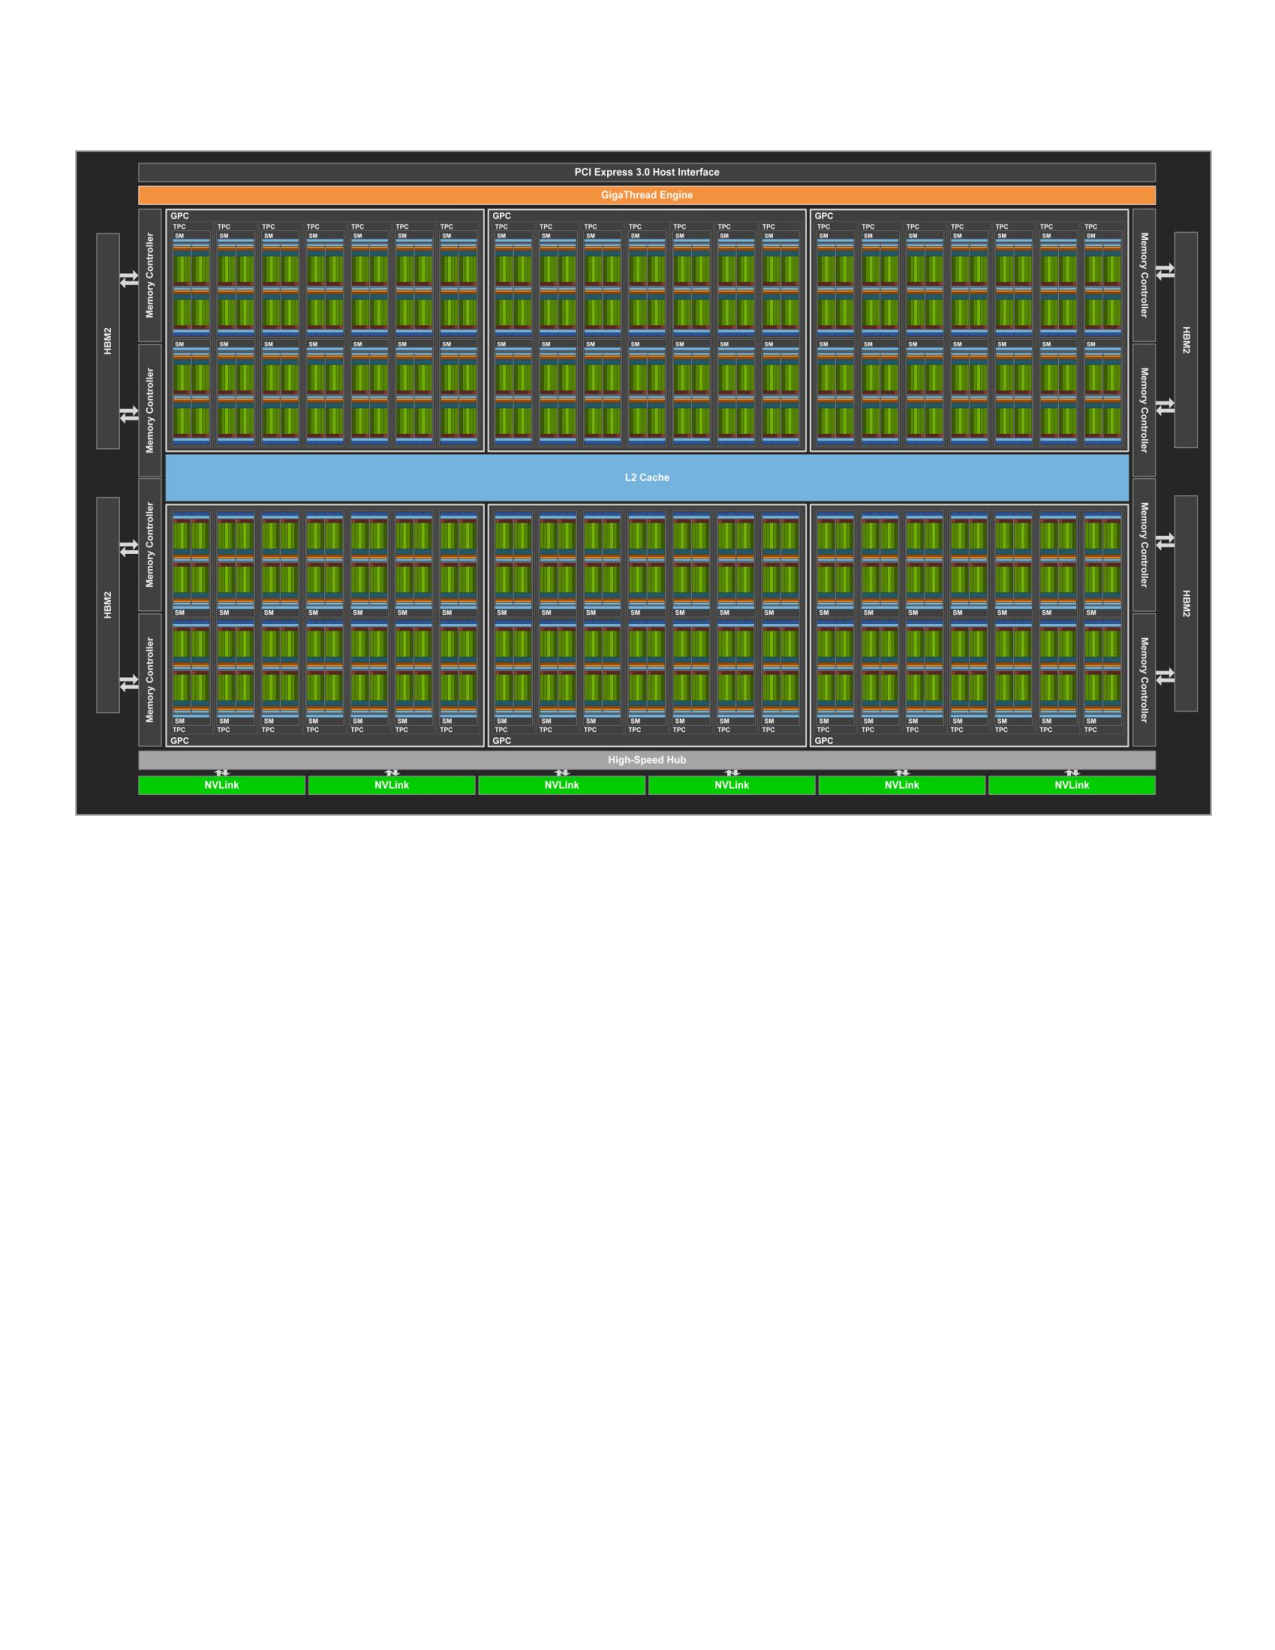
\includegraphics[width=0.8\textwidth]{figures/L24/NVIDIAVoltaV100GPUBlockDiagram.pdf}
    \caption{Block diagram for the NVIDIA Volta V100 GPU. Image source: \href{https://images.nvidia.com/content/volta-architecture/pdf/volta-architecture-whitepaper.pdf}{NVIDIA Volta V100 White Paper}.}
    \label{NVIDIAV100BlockDiagram.fig}
\end{figure}
Each core is equipped with 32 double precision floating point units per compute core as illustrated in Figure \ref{NVIDIAV100CoreDiagram.fig}. Thus the V100 has 2,560 double precision floating point units. Each of these floating point units can execute a Fused Multiply ADD (FMADD) per clock cycle. Furthermore, the clock frequency of the Volta core is dynamically clocked up to 1.53GHz. 
\begin{figure}[htbp!]
    \centering
    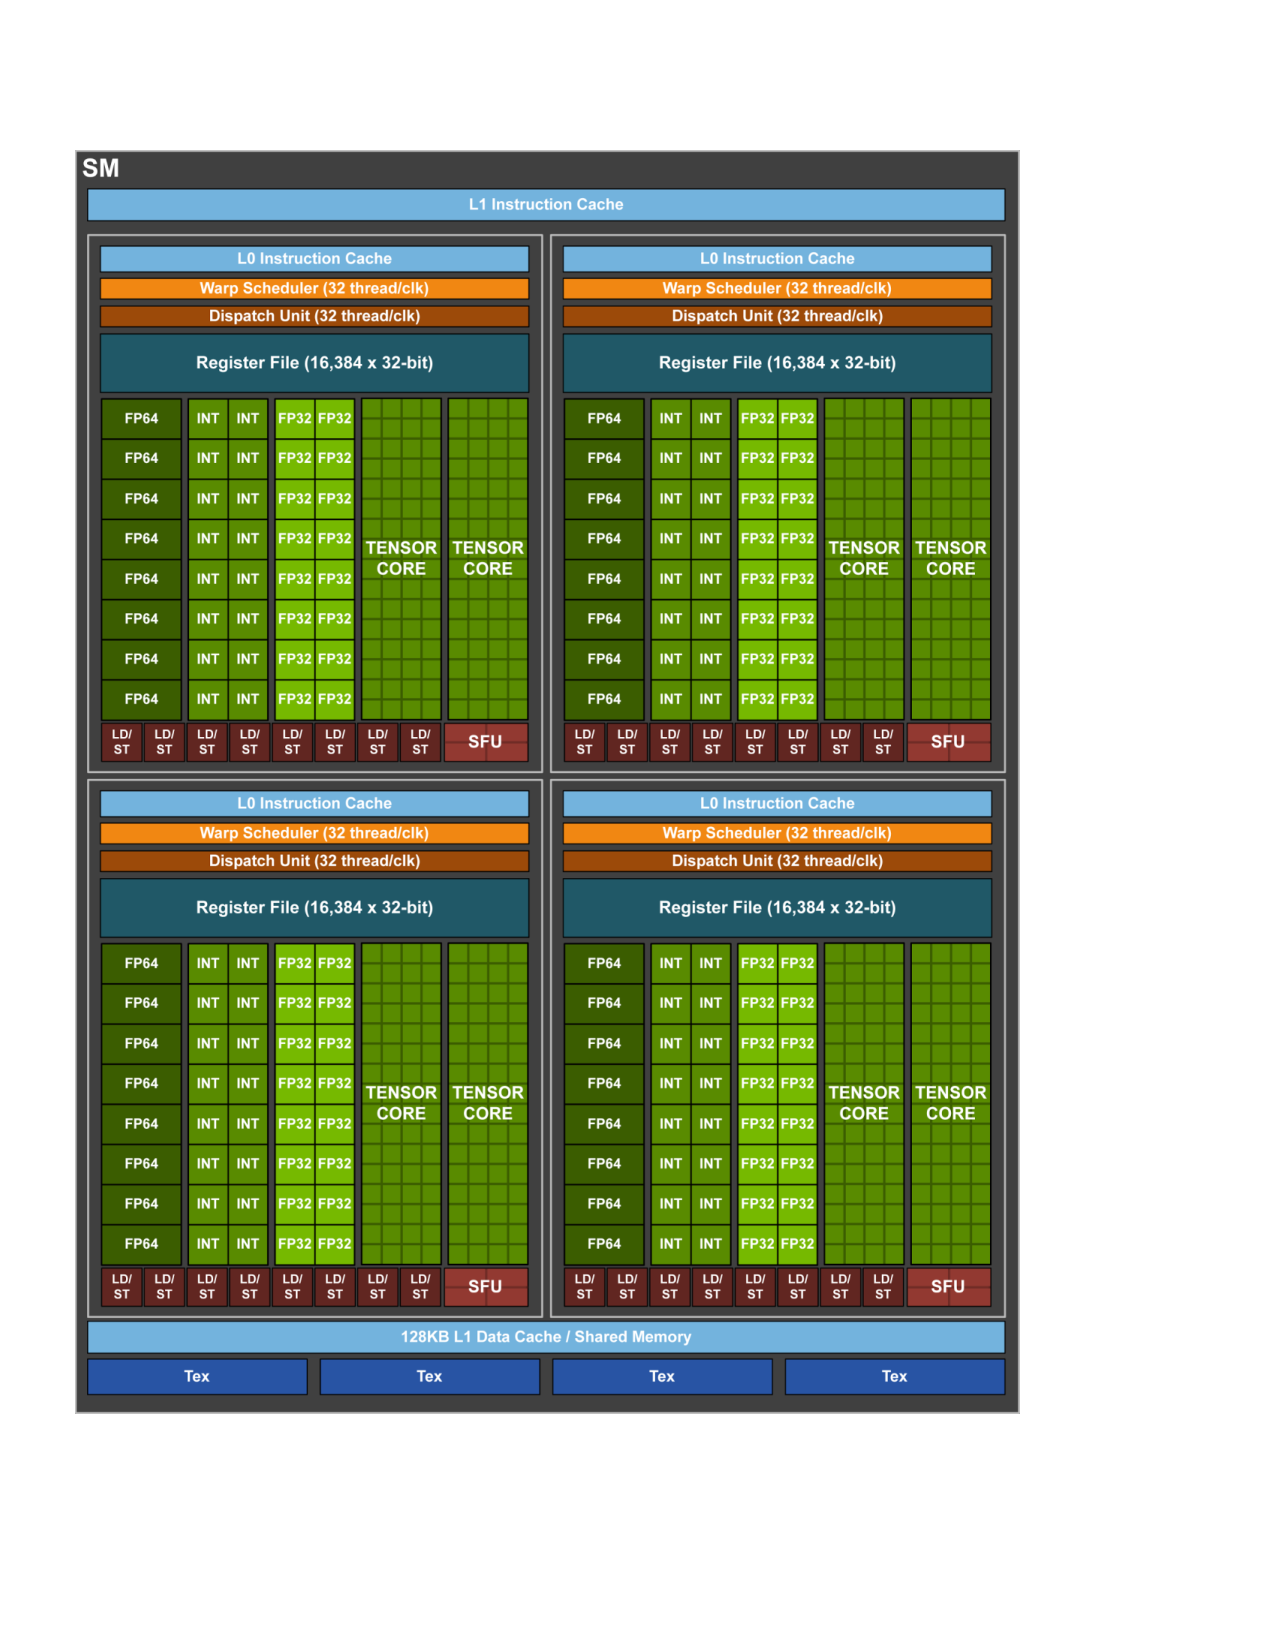
\includegraphics[width=0.66\textwidth]{figures/L24/NVIDIAVoltaV100GPUCoreDiagram.pdf}
    \caption{Core diagram for the NVIDIA Volta V100 GPU Streaming Multiprocessor. Image source: \href{https://images.nvidia.com/content/volta-architecture/pdf/volta-architecture-whitepaper.pdf}{NVIDIA Volta V100 White Paper}.}
    \label{NVIDIAV100CoreDiagram.fig}
\end{figure}
Thus the V100 can theoretically perform
\[
|\mbox{\# CORES}| \times |\mbox{\# SIMD}| \times |\mbox{\# OPS/FMADD}| \times |\mbox{FREQUENCY}| = 80 \times 32 \times 2 \times 1.53\;GHz \approx 7.8\; \mbox{TFLOPS}/s.
\]
As an aside the observant reader will notice in Figure \ref{NVIDIAV100CoreDiagram.fig} that each V100 SM also includes compute units labelled as ``TENSOR CORE''. These are highly specialized hardware for \href{https://www.nvidia.com/en-us/data-center/tensorcore/}{computing half precision (16 bit) tensor operations targeting machine learning applications}. Some researchers have coaxed these low precision tensor cores into performing more general purpose calculations using iterative refinement algorithms \cite{masliah2016high,markidis2018nvidia,haidar2018harnessing,haidar2018design,blanchard2019mixed}. By and large however many GPU enabled applications do not exploit the extra performance bumps available from the tensor cores because of their limitation to processing floating point variables with half precision.

The 32-wide SIMD units are central to the design of the GPU cores and achieve high throughput for good reason: whereas vectorization was a late addition to CPU cores it was baked into the GPU compute cores from the start. In fact until recently all operations on NVIDIA GPUs are processed as full 32-wide vector operations. Thus forcing a GPU core to perform a scalar operation is the exception rather than the norm. In fact it can be easier to write SIMD parallelized code for the GPU than for the CPU!

\section{GPU memory system}

% 3.1 memory hierarchy (stacked 3d HBM2 - what is it ?)

So far we have focused on the abundance of floating point units in modern GPUs, in particular the over provisioned NVIDIA Volta GPU. You might ask, why is it ``over provisioned'' ? The reality is that the GPU cores are routinely idled during calculations because there are so many floating point units that the GPU device system memory is unable to provide data at a fast enough rate to keep them occupied, i.e. they consume available data too fast !

To understand the imbalance between the GPU floating performance and GPU device memory capability, consider the block diagram of the NVIDIA Volta V100 shown in Figure \ref{GPUVoltaBlockMemoryDiagram.fig}. A typical Volta class GPU has up to 80 compute cores. Each equipped with just 256KB of register memory and 128KB of unified L1/shared memory. The registers, cache, and shared scratch pad have to be shared amongst 32 double precision floating point units. That means that all the data that threads need to complete their task must reside in this fast memory, otherwise they must request data load/stores from device memory. This has significant ramifications for the type of computational tasks suitable for a GPU thread. 

\begin{figure}[htbp!]
    \centering
    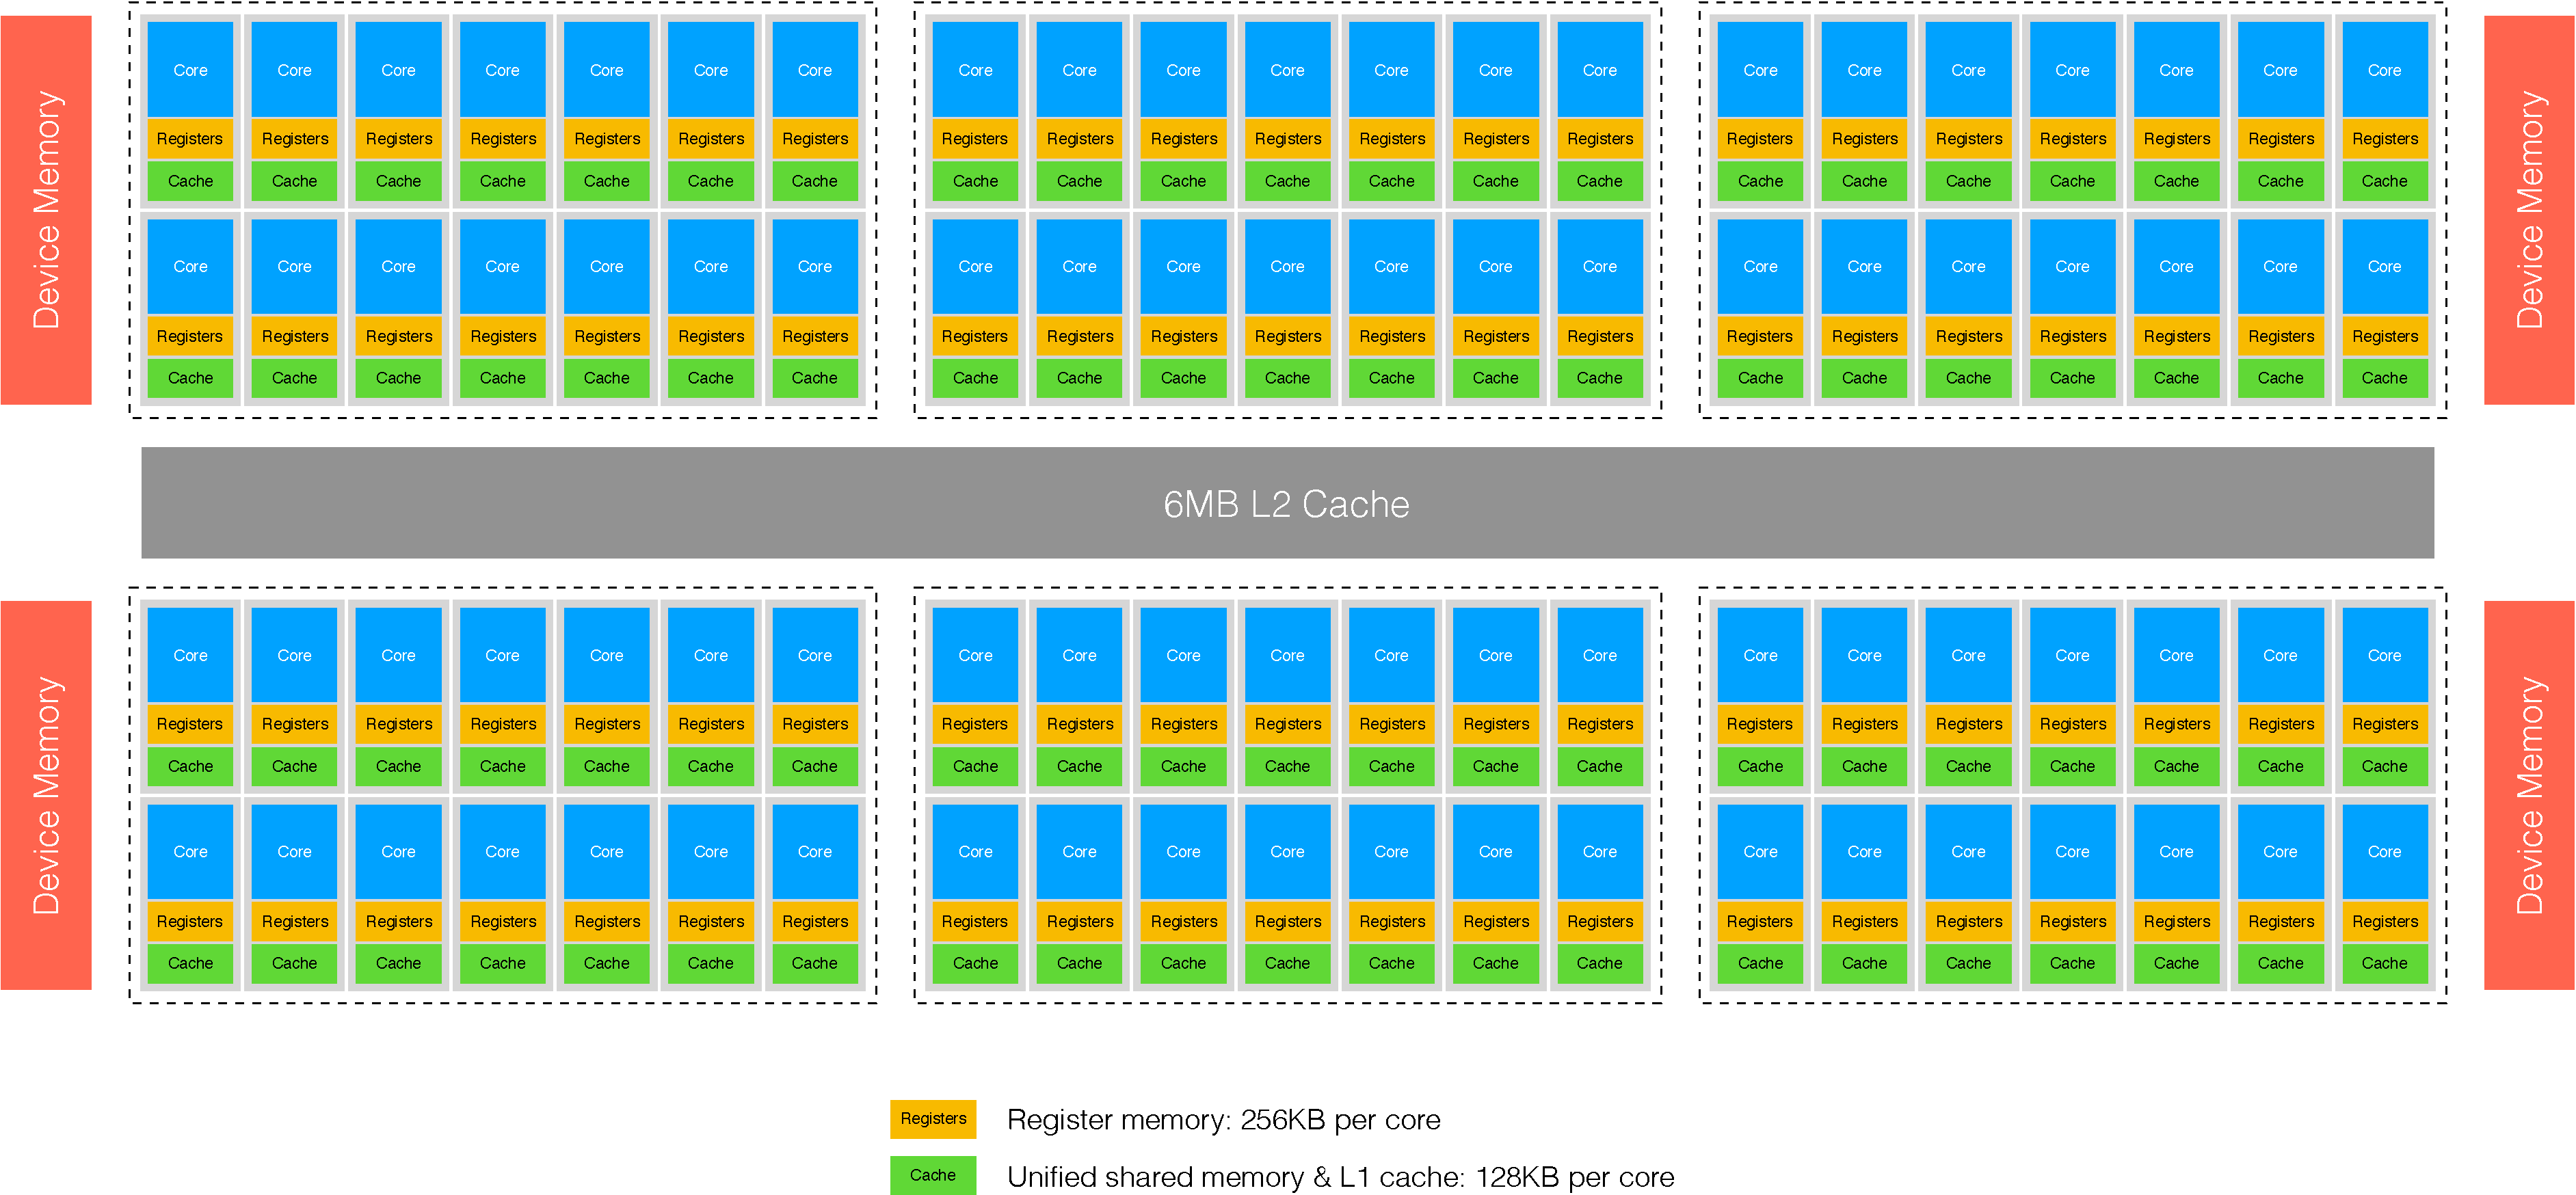
\includegraphics[width=0.85\textwidth]{figures/L24/CMDA3634FA19VoltaBlockMemory-crop.pdf}
    \caption{Block diagram of memory hierarchy of the 84 core full NVIDIA GV100 GPU.}
    \label{GPUVoltaBlockMemoryDiagram.fig}
\end{figure}


In Figure \ref{GPUFlopsPerByteTrends.fig} we show the ratio of flops per byte required to achieve peak performance when data is streamed from off-chip memory. We will refer to this ratio as the peak arithmetic intensity. 


\begin{figure}[htbp!]
    \centering
    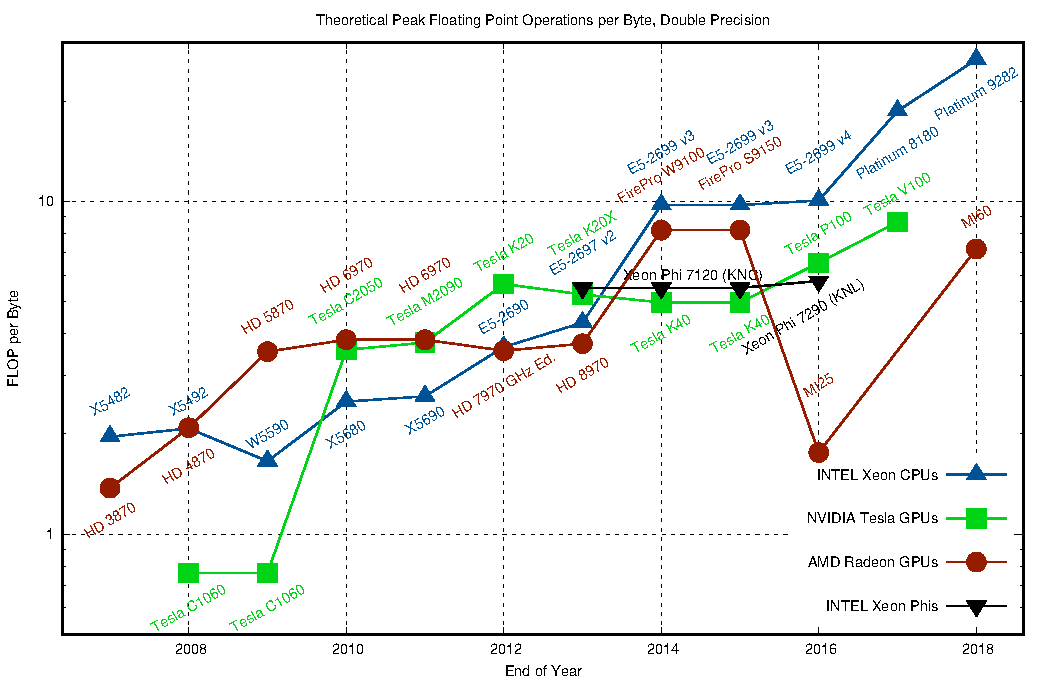
\includegraphics[width=0.66\textwidth]{figures/L24/flop-per-byte-dp.pdf}
    \caption{Trend in the number of double precision floating point operations required per byte of data to achieve peak performance. Image generated using Karl Rupp's scripts and data sourced from \href{https://github.com/karlrupp/cpu-gpu-mic-comparison}{his GitHub repository} subject to \href{https://github.com/karlrupp/cpu-gpu-mic-comparison/blob/master/LICENSE.txt}{this license}. }
    \label{GPUFlopsPerByteTrends.fig}
\end{figure}

Recent GPUs require a peak arithmetic intensity close to 10 double precision floating point operations per byte loaded or stored from off-chip memory. Very few computational tasks require an arithmetic intensity of 10. Some examples assuming double precision arithmetic are given in Table \ref{arithmeticIntensity.tab}.

\begin{table}[htbp!]
    \centering
    \small
    \begin{tabular}{l||l|c|c|l} \hline
    Operation & Math & Reads & Writes & Arithmetic intensity \\ \hline
    Add  & $z_i\leftarrow x_i+y_i$ & $2N$ & $N$ & $1/(3\times 8)\approx 0.04$ \\
    Axpy & $y_i\leftarrow \alpha x_i + y_i$ & $2N$ & $N$ & $2/(3\times 8)\approx 0.08$ \\
    Dot product & $a\leftarrow \sum_i x_iy_i$ & $2N$ & 1 &  $2/(2\times 8)\approx 0.12$\\
    Self dot product & $a\leftarrow \sum_i x_i^2$ & $N$ & $1$ & $2/(1\times 8)\approx 0.25$ \\
    Matrix-vector product & $y_i \leftarrow \alpha \sum_j A_{ij}x_j + \beta y_i$ & $N^2+2N$ & $N$ & $(2N^2+3N)/((N^2+3N)\times 8)\approx 0.25$ \\
    \hline \end{tabular}
    \normalsize
    \caption{Estimates of arithmetic intensity (floating point operations per byte of data moved) for a set of standard operations using double precision arithmetic. Reads and writes are given in terms of minimum doubles that can be read and written. Here all vectors are assumed to have $N$ entries, all matrices are assume to be of size $N\times N$, and $a,\alpha,\beta$ are all scalar variables. }
    \label{arithmeticIntensity.tab}
\end{table}
In these examples the arithmetic intensity is well below the optimal value of ten. Revisiting Figure \ref{GPUFlopsPerByteTrends.fig} in light of these practical examples and we should be rather disappointed that even a fully optimized implementation of such operations will only take advantage of a small fraction of the floating point capability of the V100. A computation with arithmetic intensity of approximately 0.1 can only extract 1\% of a GPU that requires an arithmetic intensity of about 10 to achieve peak streaming calculation performance!

\begin{figure}[htbp!]
    \centering
    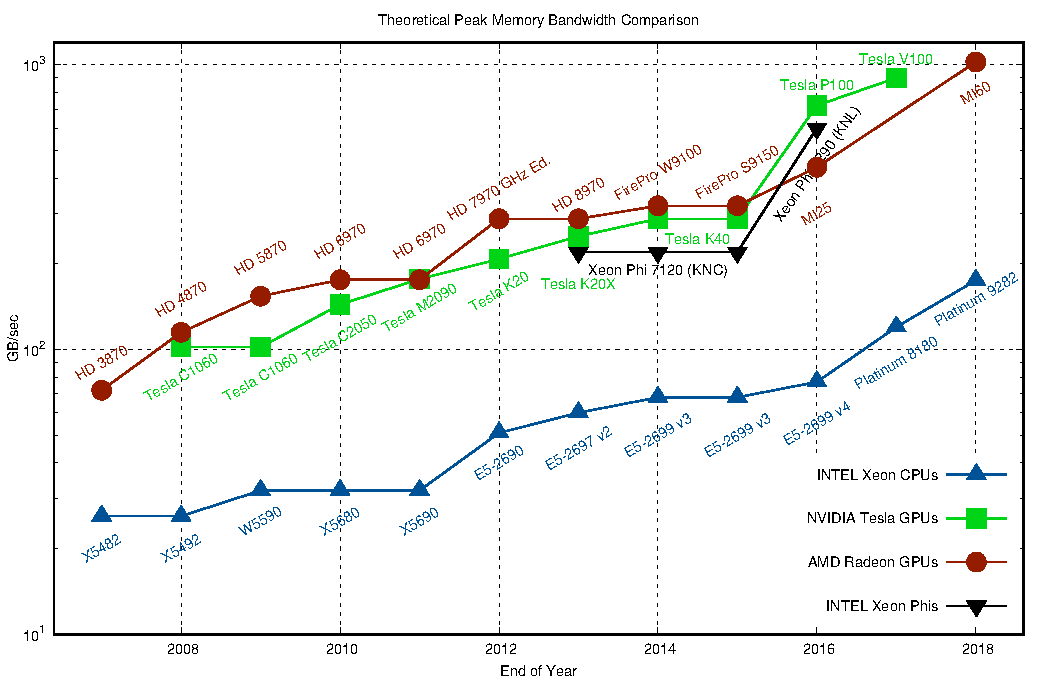
\includegraphics[width=0.66\textwidth]{figures/L24/mem-bw.pdf}
    \caption{Trend in maximum theoretical peak memory bandwidth for CPUs and GPUs over time. Image generated using Karl Rupp's scripts and data sourced from \href{https://github.com/karlrupp/cpu-gpu-mic-comparison}{his GitHub repository} subject to \href{https://github.com/karlrupp/cpu-gpu-mic-comparison/blob/master/LICENSE.txt}{this license}. }
    \label{GPUMemoryBandwidthTrends.fig}
\end{figure}

The inevitably disappointing floating point performance of these ubiquitous vector operations due to their low intinsic arithmetic intensity is not game over. In practice when presented with operations like this that are ``memory bound'' calculations we pivot. Instead of maximizing floating point performance we acknowledge that performance is limited by how fast data can be streamed through the GPU memory system and we try to maximize data throughput. In Figure \ref{GPUMemoryBandwidthTrends.fig} we show trends over time for the throughput of GPU memory systems compared to CPU memory systems. We see that there is a clear and unambiguous gap between GPU and CPU memory throughput. This is actually the secret sauce of why GPUs are gaining market share from CPUs as the computational workhorse in data centers, clusters, data processing warehouses, and super computers. The GPUs use faster memory with wider data buses than CPUs do, a trend that goes back to the earliest days when GPUs were used exclusively for rendering graphics. That task is heavily memory bound and performance depends almost entirely on the data throughput capability of the GPU's attached memory system.  

%% offload model

\section{Ongoing developments in GPU core architecture}

% 3.6.1 trends towards specialized compute elements
% 3.7 consumer cards versus compute server cards

We have seen already that the transistor counts for successive generations of GPUs has followed a version of Moore's Law. You can review the lineage of NVIDIA GPUs that precede the NVIDIA V100 card at this \href{https://en.wikipedia.org/wiki/Nvidia_Tesla}{wiki page}. The first Tesla branded GPU was the c780. In Table \ref{GPUComparison.tab} we compare with the recent NVIDIA V100 GPU to illustrate the astonishing improvements that happened between 2007 and 2017.

\begin{table}[htbp!]
    \centering
    \begin{tabular}{l||l|l} \hline
 Feature          & Tesla c780 & Tesla V100 \\ \hline
Year introduced  & 2007       & 2017 \\  \hline
Clock frequency  & 600 MHz     & 1530 MHz \\
Memory bandwidth & 78 GB/s     & 900 GB/s \\
Peak FP32 throughput  & 346 GFLOPS/s & 14,000 GFLOPS/s \\
Peak FP64 throughput  & -- & 7,000 GFLOPS/s \\ \hline
Core count & 16 & 80 \\ 
FP32 FPU per core & 8 & 64 \\
FP64 FPU per core & - & 32 \\ \hline
    \end{tabular}
    \caption{Comparison of the earliest NVIDIA server GPU, the Tesla c870 with the modern Tesla V100. Specs sourced from \href{https://www.techpowerup.com/gpu-specs/tesla-c870.c1542}{techpowerup GPU database} and \href{https://en.wikipedia.org/wiki/Nvidia_Tesla}{wiki list of NVIDIA Tesla GPUs}. }
    \label{GPUComparison.tab}
\end{table}

{\bf Note}: in a decade the floating point throughput has increased by a factor of 40 but the memory bandwidth only increased by a factor of 11. This tracks with the increase we see in the arithmetic intensity trend Figure \ref{GPUFlopsPerByteTrends.fig}. However, this is a super worrying issue when we contemplate future GPUs. The problem is that the memory throughput is increasing more slowly each generation than the floating point performance is increasing. We effectively are wasting silicon or just idling compute cores while they wait for data to arrive. 

The manufacturers have responded to the memory bandwidth gap increasing over time by resisting the urge to maximize the number of vanilla compute cores per GPU. For instance NVIDIA's latest consumer GPUs have added specialized compute units to each compute core. There are two types of specialized co-co-processors: the ray tracing core in the NVIDIA RTX GPUs  perform custom operations to accelerate scene rendering and the tensor cores in the NVIDIA Volta class GPUs and later generations perform specialized low precision matrix multiplication operations. Each of these two new types of core perform a large number of operations per input value, and furthermore open up GPU computing to new applications. Ray tracing before the advent of customized cores was not feasible for realtime rendering in games, but now Battlefield 4 and other triple A titles can run with raytracing enabled for enhanced visuals but with a reduced display framerate (to the dismay of serious gamers). The tensor cores are being used for training neural networks on cloud instances to enable deep learning with very wide neural networks. 

A cynic might observe that NVIDIA has to find new application areas to grow its potential market because the trend of everfaster and faster GPUs has stalled because of the memory bandwidth crisis.

{\bf So what's next ?}: the cost of designing and manufacturing high end processors has significantly narrowed the number of chip fabrication facilities worldwide. At the time of writing the main manufacturer of the latest 7nm based processors is the Taiwan Semiconductor Manufacturing Company (TSMC). This is used by the latest AMD GPUs and unfortunately also the latest iPhone 11 phones. The demand for the iPhone is strong and consequently the new generations of AMD GPUs will be delayed. The chalelnges of producing processors at 7nm means that there is now a supply problem and both prices and delivery times will increase. You can expect the price of your iPhone and GPUs to increase accordingly. Overall, the lack of competition in manufacturing will impact cost. But the major existential threat to next generation GPUs is the difficulty and cost of manufacturing them. 

Intel is addressing the production issues by switching from building a processor as a monolithic chip to building instead a processor as a collection of chiplets. The idea is that a chip will be constructed from a set of smaller building blocks that will cost less in design and have higher yield in production since more chiplets can be constructed from a single wafer and the cost of a dud chiplet is lower than the cost of a dud monolithic chip. 

Looking further ahead we can speculate that chips will be constructed from stacked chiplets to reduce the sprawl inherent in 2D chip design. This will need to be accompanied with memory that is collocated with the chiplets. Fingers crossed that this technology becomes viable in the near future.




\section{Examples of applications suitable for GPU acceleration}

% 2.1 purpose (bitcoin, crypto, machine learning)
% 2.2 market
% 2.3 accelerator/off-load model

% 3.4 performance trends


% 4. GPU applications (including TW apps)
% 4.1 FEM 
% 4.2 Seismic FDTD
% 4.3 DG
% 4.4 Flow calculations
% 4.5 ML/tensor-flow

\section{GPUs and super-computing}

% 5. mega systems 
% 5.1 DOE systems
% 5.2 AWS/Google Cloud/GPU Eater/Azure instances (prices, models)
% 5.3 ECP
% 5.4 top 500 lists

\section{GPU programming models}

% 6. programming models (stress offload computing)
% 6.1 CUDA (maybe pre-CUDA)
% 6.2 OpenCL
% 6.3 OpenACC
% 6.4 HIP
% 6.5 vendor preferred solutions
% 6.6 OCCA ?

% 7.  Math libraries
% 7.1 https://developer.nvidia.com/gpu-accelerated-libraries

 GPUs have also transitioned to general purpose computing devices. At inception GPUs were viewed as niche products suitable for gaming and rendering on graphics workstations. But since the mid 2000s they have been adapted to more general purpose computing applications. This coincides with the so-called end of Dennard scaling around 2005 when increasing CPU processor clock frequencies hit the thermal wall. Suddenly there was an opportunity for competition in the processor space since applications were no longer sped up just by buying the latest Intel or AMD CPU. Furthermore, software developers were having limited success squeezing good performance out of the new multi-core CPUs. 

In 2007-2008 NVIDIA released  GPUs with new compute capabilities and a new programming model called the Compute Unified Device Architecture (CUDA) to exploit the new hardware features. Researchers found that if they ported their applications to CUDA that they could get remarkable speed ups. In part this was due to higher peak performance and higher memory throughput, but the performance bumps  in many instances could be attributed to the key feature that the GPU is ab initio parallel in core and vectorization. Whereas developers struggled to persuade compilers to generate SIMD parallel code for CPUs, they couldn't help but generate SIMD parallel code when writing CUDA code at least if they paid a modicum of attention to the GPU architecture and CUDA language features. In the following lectures we will describe the CUDA programming language and add more detail to inform your mental model of a modern GPU architecture.

%% OpenCL, HIP, diagram ? 
%% which language for which GPU/CPU ?
%% portability ?

\section{GPU computing references}

We list some books that are useful sources of introduction material. The thumbs up are my personal assessment of the texts.

{\bf Presentations about GPUs}:

{\bf CUDA books}:

\begin{enumerate}
    \item \cite{sanders2010cuda}: from the blurb ``\emph{CUDA now brings this valuable resource to programmers working on applications in other domains, including science, engineering, and finance. No knowledge of graphics programming is required; just the ability to program in a modestly extended version of C. CUDA by Example, written by two senior members of the CUDA software platform team, shows programmers how to employ this new technology. The authors introduce each area of CUDA development through working examples. After a concise introduction to the CUDA platform and architecture, as well as a quick-start guide to CUDA C, the book details the techniques and trade-offs associated with each key CUDA feature}.'' (\faThumbsOUp{}\faThumbsOUp{})
    
    \item \cite{kindratenko2014numerical}: from the blurb ``\emph{This book is intended to serve as a practical guide for the development and implementation of numerical algorithms on Graphics Processing Units (GPUs). The book assumes that the 
    reader is familiar with the mathematical context and has a good working knowledge of GPU}.'' (\faThumbsOUp{}\faThumbsOUp{} and available via \href{https://link.springer.com/content/pdf/10.1007/978-3-319-06548-9.pdf}{SpringerLink})
    
    \item \cite{farber2011cuda}: from the blurb ``\emph{In addition, the book provides many case studies, which are used to explain and reinforce important GPU concepts like CUDA threads, the GPU memory hierarchy, and scalability across multiple GPUs including an MPI example }'' (\faThumbsOUp{})
    
    \item \cite{cheng2014professional}: from the blurb ``\emph{Designed for professionals across multiple industrial sectors, Professional CUDA C Programming  presents CUDA -- a parallel computing platform and programming model designed to ease the development of GPU programming -- fundamentals in an easy-to-follow format, and teaches readers how to think in parallel and implement parallel algorithms on GPUs}'' (\faThumbsOUp{})
    
    \item \cite{kirk2016programming}: from the blurb ``\emph{\ldots shows both student and professional alike the basic concepts of parallel programming and GPU architecture, exploring, in detail, various techniques for constructing parallel programs.}'' (\faThumbsOUp{}\faThumbsOUp{}\faThumbsOUp{}) 
    
\end{enumerate}

{\bf OpenCL books}:

\begin{enumerate}
    \item \cite{gaster2012heterogeneous}: from the blurb ``\emph{ \ldots teaches OpenCL and parallel programming for complex systems that may include a variety of device architectures: multi-core CPUs, GPUs, and fully-integrated Accelerated Processing Units (APUs) such as AMD Fusion technology. It is the first textbook that presents OpenCL programming appropriate for the classroom and is intended to support a parallel programming course. }'' (\faThumbsOUp{})
\end{enumerate}

\section{Summary of GPU computing}


\printbibliography[heading=subbibliography]